\documentclass[]{article}
\usepackage{lmodern}
\usepackage{amssymb,amsmath}
\usepackage{ifxetex,ifluatex}
\usepackage{fixltx2e} % provides \textsubscript
\ifnum 0\ifxetex 1\fi\ifluatex 1\fi=0 % if pdftex
  \usepackage[T1]{fontenc}
  \usepackage[utf8]{inputenc}
\else % if luatex or xelatex
  \ifxetex
    \usepackage{mathspec}
  \else
    \usepackage{fontspec}
  \fi
  \defaultfontfeatures{Ligatures=TeX,Scale=MatchLowercase}
\fi
% use upquote if available, for straight quotes in verbatim environments
\IfFileExists{upquote.sty}{\usepackage{upquote}}{}
% use microtype if available
\IfFileExists{microtype.sty}{%
\usepackage{microtype}
\UseMicrotypeSet[protrusion]{basicmath} % disable protrusion for tt fonts
}{}
\usepackage[margin=1in]{geometry}
\usepackage{hyperref}
\hypersetup{unicode=true,
            pdftitle={Qualifying Exam 2019},
            pdfauthor={Exam \#7},
            pdfborder={0 0 0},
            breaklinks=true}
\urlstyle{same}  % don't use monospace font for urls
\usepackage{color}
\usepackage{fancyvrb}
\newcommand{\VerbBar}{|}
\newcommand{\VERB}{\Verb[commandchars=\\\{\}]}
\DefineVerbatimEnvironment{Highlighting}{Verbatim}{commandchars=\\\{\}}
% Add ',fontsize=\small' for more characters per line
\usepackage{framed}
\definecolor{shadecolor}{RGB}{248,248,248}
\newenvironment{Shaded}{\begin{snugshade}}{\end{snugshade}}
\newcommand{\AlertTok}[1]{\textcolor[rgb]{0.94,0.16,0.16}{#1}}
\newcommand{\AnnotationTok}[1]{\textcolor[rgb]{0.56,0.35,0.01}{\textbf{\textit{#1}}}}
\newcommand{\AttributeTok}[1]{\textcolor[rgb]{0.77,0.63,0.00}{#1}}
\newcommand{\BaseNTok}[1]{\textcolor[rgb]{0.00,0.00,0.81}{#1}}
\newcommand{\BuiltInTok}[1]{#1}
\newcommand{\CharTok}[1]{\textcolor[rgb]{0.31,0.60,0.02}{#1}}
\newcommand{\CommentTok}[1]{\textcolor[rgb]{0.56,0.35,0.01}{\textit{#1}}}
\newcommand{\CommentVarTok}[1]{\textcolor[rgb]{0.56,0.35,0.01}{\textbf{\textit{#1}}}}
\newcommand{\ConstantTok}[1]{\textcolor[rgb]{0.00,0.00,0.00}{#1}}
\newcommand{\ControlFlowTok}[1]{\textcolor[rgb]{0.13,0.29,0.53}{\textbf{#1}}}
\newcommand{\DataTypeTok}[1]{\textcolor[rgb]{0.13,0.29,0.53}{#1}}
\newcommand{\DecValTok}[1]{\textcolor[rgb]{0.00,0.00,0.81}{#1}}
\newcommand{\DocumentationTok}[1]{\textcolor[rgb]{0.56,0.35,0.01}{\textbf{\textit{#1}}}}
\newcommand{\ErrorTok}[1]{\textcolor[rgb]{0.64,0.00,0.00}{\textbf{#1}}}
\newcommand{\ExtensionTok}[1]{#1}
\newcommand{\FloatTok}[1]{\textcolor[rgb]{0.00,0.00,0.81}{#1}}
\newcommand{\FunctionTok}[1]{\textcolor[rgb]{0.00,0.00,0.00}{#1}}
\newcommand{\ImportTok}[1]{#1}
\newcommand{\InformationTok}[1]{\textcolor[rgb]{0.56,0.35,0.01}{\textbf{\textit{#1}}}}
\newcommand{\KeywordTok}[1]{\textcolor[rgb]{0.13,0.29,0.53}{\textbf{#1}}}
\newcommand{\NormalTok}[1]{#1}
\newcommand{\OperatorTok}[1]{\textcolor[rgb]{0.81,0.36,0.00}{\textbf{#1}}}
\newcommand{\OtherTok}[1]{\textcolor[rgb]{0.56,0.35,0.01}{#1}}
\newcommand{\PreprocessorTok}[1]{\textcolor[rgb]{0.56,0.35,0.01}{\textit{#1}}}
\newcommand{\RegionMarkerTok}[1]{#1}
\newcommand{\SpecialCharTok}[1]{\textcolor[rgb]{0.00,0.00,0.00}{#1}}
\newcommand{\SpecialStringTok}[1]{\textcolor[rgb]{0.31,0.60,0.02}{#1}}
\newcommand{\StringTok}[1]{\textcolor[rgb]{0.31,0.60,0.02}{#1}}
\newcommand{\VariableTok}[1]{\textcolor[rgb]{0.00,0.00,0.00}{#1}}
\newcommand{\VerbatimStringTok}[1]{\textcolor[rgb]{0.31,0.60,0.02}{#1}}
\newcommand{\WarningTok}[1]{\textcolor[rgb]{0.56,0.35,0.01}{\textbf{\textit{#1}}}}
\usepackage{longtable,booktabs}
\usepackage{graphicx,grffile}
\makeatletter
\def\maxwidth{\ifdim\Gin@nat@width>\linewidth\linewidth\else\Gin@nat@width\fi}
\def\maxheight{\ifdim\Gin@nat@height>\textheight\textheight\else\Gin@nat@height\fi}
\makeatother
% Scale images if necessary, so that they will not overflow the page
% margins by default, and it is still possible to overwrite the defaults
% using explicit options in \includegraphics[width, height, ...]{}
\setkeys{Gin}{width=\maxwidth,height=\maxheight,keepaspectratio}
\IfFileExists{parskip.sty}{%
\usepackage{parskip}
}{% else
\setlength{\parindent}{0pt}
\setlength{\parskip}{6pt plus 2pt minus 1pt}
}
\setlength{\emergencystretch}{3em}  % prevent overfull lines
\providecommand{\tightlist}{%
  \setlength{\itemsep}{0pt}\setlength{\parskip}{0pt}}
\setcounter{secnumdepth}{0}
% Redefines (sub)paragraphs to behave more like sections
\ifx\paragraph\undefined\else
\let\oldparagraph\paragraph
\renewcommand{\paragraph}[1]{\oldparagraph{#1}\mbox{}}
\fi
\ifx\subparagraph\undefined\else
\let\oldsubparagraph\subparagraph
\renewcommand{\subparagraph}[1]{\oldsubparagraph{#1}\mbox{}}
\fi

%%% Use protect on footnotes to avoid problems with footnotes in titles
\let\rmarkdownfootnote\footnote%
\def\footnote{\protect\rmarkdownfootnote}

%%% Change title format to be more compact
\usepackage{titling}

% Create subtitle command for use in maketitle
\providecommand{\subtitle}[1]{
  \posttitle{
    \begin{center}\large#1\end{center}
    }
}

\setlength{\droptitle}{-2em}

  \title{Qualifying Exam 2019}
    \pretitle{\vspace{\droptitle}\centering\huge}
  \posttitle{\par}
    \author{Exam \#7}
    \preauthor{\centering\large\emph}
  \postauthor{\par}
      \predate{\centering\large\emph}
  \postdate{\par}
    \date{6/1/2019}


\begin{document}
\maketitle

\hypertarget{question-1}{%
\section{Question 1}\label{question-1}}

\hypertarget{a-number-of-meals-involving-fish-as-a-positive-test}{%
\subsection{a) Number of meals involving fish as a positive
test}\label{a-number-of-meals-involving-fish-as-a-positive-test}}

\begin{Shaded}
\begin{Highlighting}[]
\CommentTok{# epiR package for calculating sensitivity and specificity}
\NormalTok{sensspec0 <-}\StringTok{ }\KeywordTok{epi.tests}\NormalTok{(ctable0)}
\NormalTok{sensspec1 <-}\StringTok{ }\KeywordTok{epi.tests}\NormalTok{(ctable1)}
\NormalTok{sensspec2 <-}\StringTok{ }\KeywordTok{epi.tests}\NormalTok{(ctable2)}
\NormalTok{sensspec3 <-}\StringTok{ }\KeywordTok{epi.tests}\NormalTok{(ctable3)}
\NormalTok{sensspec4 <-}\StringTok{ }\KeywordTok{epi.tests}\NormalTok{(ctable4)}
\NormalTok{sensspec7 <-}\StringTok{ }\KeywordTok{epi.tests}\NormalTok{(ctable7)}
\NormalTok{sensspec14 <-}\StringTok{ }\KeywordTok{epi.tests}\NormalTok{(ctable14)}
\NormalTok{sensspec21 <-}\StringTok{ }\KeywordTok{epi.tests}\NormalTok{(ctable21)}
\end{Highlighting}
\end{Shaded}

\begin{longtable}[]{@{}lrr@{}}
\toprule
& Sensitivity & Specificity\tabularnewline
\midrule
\endhead
\textgreater{}=0 & 100 & 0.0\tabularnewline
\textgreater{}=1 & 100 & 8.0\tabularnewline
\textgreater{}=2 & 100 & 19.2\tabularnewline
\textgreater{}=3 & 100 & 28.0\tabularnewline
\textgreater{}=4 & 90 & 28.8\tabularnewline
\textgreater{}=7 & 70 & 36.8\tabularnewline
\textgreater{}=14 & 30 & 89.6\tabularnewline
\textgreater{}=21 & 30 & 93.6\tabularnewline
\bottomrule
\end{longtable}

\hypertarget{b-appropriate-thresholds}{%
\subsection{b) Appropriate thresholds}\label{b-appropriate-thresholds}}

Sensitivity refers to the true positive rate, or the probability that a
test will rule in disease correctly. Specificity indicates the true
negative rate, or the probability that a test will correctly rule out
disease. Therefore, the probability of a false negative is 100 -
sensitivity and the the false positive rate is 100 - specificity.

\hypertarget{i.-true-positives}{%
\subsubsection{i. True positives}\label{i.-true-positives}}

If we want to maximize true positives while minimizing false positives,
the optimal threshold is the one with the highest sensitivity and lowest
100 - specificity. A threshold of \textgreater{}= 3 meals per week
including fish would provide a 100\% true positive rate and a 72\% false
negative rate.

\hypertarget{ii.-true-negatives}{%
\subsubsection{ii. True negatives}\label{ii.-true-negatives}}

Maximizing true negatives first and then true positives requires
choosing the test with highest specificity and highest sensitivity. In
this case a threshold of \textgreater{}= 21 meals including fish per
week would provide a true negative detection rate of 93.6\% and a true
positive rate of 30\%.

\hypertarget{c-bootstrap-sampling-for-21-meals-threshold}{%
\subsection{c) Bootstrap sampling for \textgreater{}= 21 meals
threshold}\label{c-bootstrap-sampling-for-21-meals-threshold}}

\begin{Shaded}
\begin{Highlighting}[]
\CommentTok{# Vector for storing results}
\KeywordTok{set.seed}\NormalTok{(}\DecValTok{1234}\NormalTok{)}
\NormalTok{B <-}\StringTok{ }\DecValTok{10000}
\NormalTok{sens_results <-}\StringTok{ }\KeywordTok{numeric}\NormalTok{(B)}
\NormalTok{spec_results <-}\StringTok{ }\KeywordTok{numeric}\NormalTok{(B)}
\CommentTok{# Loop}
\ControlFlowTok{for}\NormalTok{ (i }\ControlFlowTok{in} \DecValTok{1}\OperatorTok{:}\NormalTok{B) \{}
\NormalTok{  meals <-}\StringTok{ }\KeywordTok{sample}\NormalTok{(fish}\OperatorTok{$}\NormalTok{fishmlwk,}\DataTypeTok{replace =}\NormalTok{ T)}
\NormalTok{  meals <-}\StringTok{ }\KeywordTok{ifelse}\NormalTok{(meals }\OperatorTok{>=}\StringTok{ }\DecValTok{21}\NormalTok{,}\DecValTok{1}\NormalTok{,}\DecValTok{0}\NormalTok{)}
\NormalTok{  response <-}\StringTok{ }\KeywordTok{sample}\NormalTok{(fish}\OperatorTok{$}\NormalTok{MeHg,}\DataTypeTok{replace =}\NormalTok{ T)}
\NormalTok{  response <-}\StringTok{ }\KeywordTok{ifelse}\NormalTok{(response }\OperatorTok{>=}\StringTok{ }\DecValTok{8}\NormalTok{,}\DecValTok{1}\NormalTok{,}\DecValTok{0}\NormalTok{)}
\NormalTok{  table <-}\StringTok{ }\KeywordTok{table}\NormalTok{(}\KeywordTok{factor}\NormalTok{(meals,}\DataTypeTok{levels=}\DecValTok{1}\OperatorTok{:}\DecValTok{0}\NormalTok{),}\KeywordTok{factor}\NormalTok{(response,}\DataTypeTok{levels=}\DecValTok{1}\OperatorTok{:}\DecValTok{0}\NormalTok{))}
\NormalTok{  sens_results[i] <-}\StringTok{ }\NormalTok{(table[}\DecValTok{1}\NormalTok{,}\DecValTok{1}\NormalTok{]}\OperatorTok{/}\KeywordTok{sum}\NormalTok{(table[,}\DecValTok{1}\NormalTok{])) }\OperatorTok{*}\StringTok{ }\DecValTok{100}
\NormalTok{  spec_results[i] <-}\StringTok{ }\NormalTok{(table[}\DecValTok{2}\NormalTok{,}\DecValTok{2}\NormalTok{]}\OperatorTok{/}\KeywordTok{sum}\NormalTok{(table[,}\DecValTok{2}\NormalTok{])) }\OperatorTok{*}\StringTok{ }\DecValTok{100}
\NormalTok{\}}
\end{Highlighting}
\end{Shaded}

\hypertarget{i.-plots}{%
\subsubsection{i. Plots}\label{i.-plots}}

\begin{Shaded}
\begin{Highlighting}[]
\CommentTok{# Plots}
\KeywordTok{hist}\NormalTok{(sens_results,}\DataTypeTok{main =} \StringTok{"Sensitivity Bootstrap Distribution"}\NormalTok{,}\DataTypeTok{xlab =} \StringTok{"Sensitivity"}\NormalTok{)}
\end{Highlighting}
\end{Shaded}

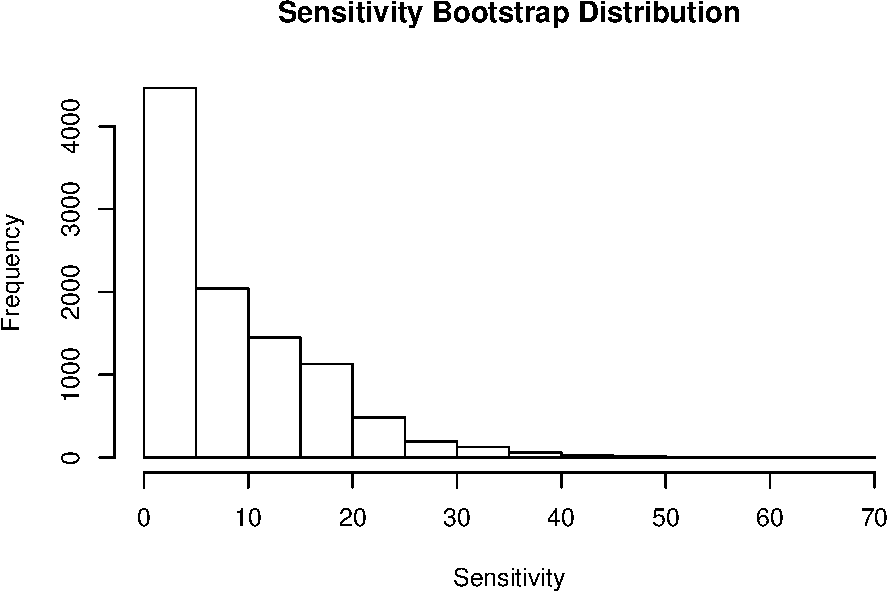
\includegraphics{QE2019_files/figure-latex/unnamed-chunk-6-1.pdf}

\begin{Shaded}
\begin{Highlighting}[]
\KeywordTok{hist}\NormalTok{(spec_results,}\DataTypeTok{main =} \StringTok{"Specificity Bootstrap Distribution"}\NormalTok{,}\DataTypeTok{xlab =} \StringTok{"Specificity"}\NormalTok{)}
\end{Highlighting}
\end{Shaded}

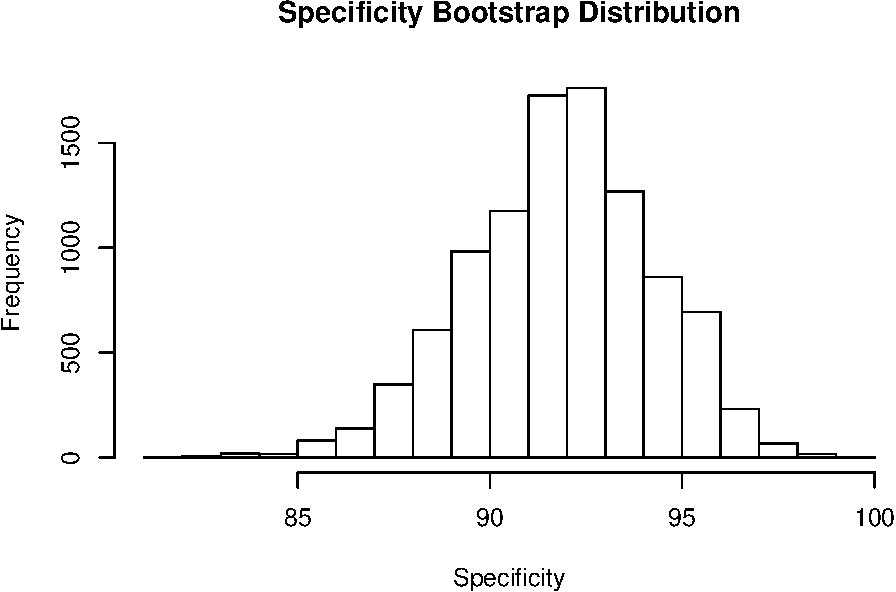
\includegraphics{QE2019_files/figure-latex/unnamed-chunk-6-2.pdf}

\hypertarget{ii.-mean-se-and-bias-from-bootstrap-distributions}{%
\subsubsection{ii. Mean, SE, and Bias From Bootstrap
Distributions}\label{ii.-mean-se-and-bias-from-bootstrap-distributions}}

\begin{longtable}[]{@{}lrrr@{}}
\toprule
& Mean & Standard Error & Bias\tabularnewline
\midrule
\endhead
Sensitivity & 8.16521 & 0.0922186 & -21.83479\tabularnewline
Specificity & 91.87575 & 0.0240551 & -1.72425\tabularnewline
\bottomrule
\end{longtable}

\hypertarget{iii.-90-bootstrap-and-normal-percentile-confidence-intervals}{%
\subsubsection{iii. 90\% Bootstrap and Normal Percentile Confidence
Intervals}\label{iii.-90-bootstrap-and-normal-percentile-confidence-intervals}}

\begin{Shaded}
\begin{Highlighting}[]
\CommentTok{# Sensitivity}
\CommentTok{# Normal percentiles}
\NormalTok{L <-}\StringTok{ }\KeywordTok{mean}\NormalTok{(sens_results) }\OperatorTok{-}\StringTok{ }\NormalTok{(}\FloatTok{1.645} \OperatorTok{*}\StringTok{ }\KeywordTok{sd}\NormalTok{(sens_results))}
\NormalTok{L}
\end{Highlighting}
\end{Shaded}

\begin{verbatim}
## [1] -7.004749
\end{verbatim}

\begin{Shaded}
\begin{Highlighting}[]
\NormalTok{U <-}\StringTok{ }\KeywordTok{mean}\NormalTok{(sens_results) }\OperatorTok{+}\StringTok{ }\NormalTok{(}\FloatTok{1.645} \OperatorTok{*}\StringTok{ }\KeywordTok{sd}\NormalTok{(sens_results))}
\NormalTok{U}
\end{Highlighting}
\end{Shaded}

\begin{verbatim}
## [1] 23.33517
\end{verbatim}

\begin{Shaded}
\begin{Highlighting}[]
\CommentTok{# Coverage}
\KeywordTok{sum}\NormalTok{(sens_results }\OperatorTok{<}\StringTok{ }\NormalTok{L)}\OperatorTok{/}\NormalTok{B}
\end{Highlighting}
\end{Shaded}

\begin{verbatim}
## [1] 0
\end{verbatim}

\begin{Shaded}
\begin{Highlighting}[]
\KeywordTok{sum}\NormalTok{(sens_results }\OperatorTok{>}\StringTok{ }\NormalTok{U)}\OperatorTok{/}\NormalTok{B}
\end{Highlighting}
\end{Shaded}

\begin{verbatim}
## [1] 0.0671
\end{verbatim}

\begin{Shaded}
\begin{Highlighting}[]
\CommentTok{# Bootstrap percentiles}
\KeywordTok{quantile}\NormalTok{(sens_results,}\KeywordTok{c}\NormalTok{(}\FloatTok{0.05}\NormalTok{,}\FloatTok{0.95}\NormalTok{))}
\end{Highlighting}
\end{Shaded}

\begin{verbatim}
##  5% 95% 
##   0  25
\end{verbatim}

The bootstrap distribution for sensitivity is not at all normal. The
90\% confidence interval for this distribution using normal percentiles
is (-7.00\%,23.34\%), which does not make sense as sensitivity cannot be
negative. Also, none of the bootstrap values were below the lower limit
(again, because this is impossible), when we'd expect that 5\% would be
for a normal distribution. So in this case it would probably be better
to use the bootstrap confidence interval (0\%,25\%).

\begin{Shaded}
\begin{Highlighting}[]
\CommentTok{# Specificity}
\CommentTok{# Normal percentiles}
\NormalTok{Lc <-}\StringTok{ }\KeywordTok{mean}\NormalTok{(spec_results) }\OperatorTok{-}\StringTok{ }\NormalTok{(}\FloatTok{1.645} \OperatorTok{*}\StringTok{ }\KeywordTok{sd}\NormalTok{(spec_results))}
\NormalTok{Lc}
\end{Highlighting}
\end{Shaded}

\begin{verbatim}
## [1] 87.91868
\end{verbatim}

\begin{Shaded}
\begin{Highlighting}[]
\NormalTok{Uc <-}\StringTok{ }\KeywordTok{mean}\NormalTok{(spec_results) }\OperatorTok{+}\StringTok{ }\NormalTok{(}\FloatTok{1.645} \OperatorTok{*}\StringTok{ }\KeywordTok{sd}\NormalTok{(spec_results))}
\NormalTok{Uc}
\end{Highlighting}
\end{Shaded}

\begin{verbatim}
## [1] 95.83282
\end{verbatim}

\begin{Shaded}
\begin{Highlighting}[]
\CommentTok{# Coverage}
\KeywordTok{sum}\NormalTok{(spec_results }\OperatorTok{<}\StringTok{ }\NormalTok{Lc)}\OperatorTok{/}\NormalTok{B}
\end{Highlighting}
\end{Shaded}

\begin{verbatim}
## [1] 0.0558
\end{verbatim}

\begin{Shaded}
\begin{Highlighting}[]
\KeywordTok{sum}\NormalTok{(spec_results }\OperatorTok{>}\StringTok{ }\NormalTok{Uc)}\OperatorTok{/}\NormalTok{B}
\end{Highlighting}
\end{Shaded}

\begin{verbatim}
## [1] 0.049
\end{verbatim}

\begin{Shaded}
\begin{Highlighting}[]
\CommentTok{# Bootstrap percentiles}
\KeywordTok{quantile}\NormalTok{(spec_results,}\KeywordTok{c}\NormalTok{(}\FloatTok{0.05}\NormalTok{,}\FloatTok{0.95}\NormalTok{))}
\end{Highlighting}
\end{Shaded}

\begin{verbatim}
##       5%      95% 
## 87.80488 95.79832
\end{verbatim}

The bootstrap distribution for specificity appears to be much closer to
normal than sensitivity. The 90\% normal percentile confidence interval
is (87.92\%,95.83\%), which matches the bootstrap confidence interval
very closely (87.80\%,95.80\%). Also, approximately 5\% percent of the
bootstrap values were below the lower limit and above the upper limit,
which is what we would expect from a normal distribution.

\hypertarget{d.-90-confidence-intervals-using-exact-and-asymptotic-methods}{%
\subsection{d. 90\% Confidence Intervals Using Exact and Asymptotic
Methods}\label{d.-90-confidence-intervals-using-exact-and-asymptotic-methods}}

\hypertarget{i.-sensitivity}{%
\subsubsection{i. Sensitivity}\label{i.-sensitivity}}

Clopper-Pearson Method

\[
\hat{p} = \frac{3}{10}
\]

\[
\text{CI} = (\frac{x}{x+(n-x+1)F_{1-\frac{\alpha}{2};2(n-x+1),2x}},\frac{(x+1)F_{1-\frac{\alpha}{2};2(x+1),2(n-x)}}{(n-x)+(x+1)F_{1-\frac{\alpha}{2};2(x+1),2(n-x)}})
\]

\begin{Shaded}
\begin{Highlighting}[]
\NormalTok{n <-}\StringTok{ }\KeywordTok{sum}\NormalTok{(ctable21[,}\DecValTok{1}\NormalTok{])}
\NormalTok{x <-}\StringTok{ }\NormalTok{ctable21[}\DecValTok{1}\NormalTok{,}\DecValTok{1}\NormalTok{]}
\NormalTok{L <-}\StringTok{ }\NormalTok{x}\OperatorTok{/}\NormalTok{(x}\OperatorTok{+}\NormalTok{((n}\OperatorTok{-}\NormalTok{x}\OperatorTok{+}\DecValTok{1}\NormalTok{)}\OperatorTok{*}\KeywordTok{qf}\NormalTok{(}\FloatTok{0.95}\NormalTok{,(}\DecValTok{2}\OperatorTok{*}\NormalTok{(n}\OperatorTok{-}\NormalTok{x}\OperatorTok{+}\DecValTok{1}\NormalTok{)),}\DecValTok{2}\OperatorTok{*}\NormalTok{x))) }\OperatorTok{*}\StringTok{ }\DecValTok{100}
\NormalTok{L}
\end{Highlighting}
\end{Shaded}

\begin{verbatim}
## [1] 8.726443
\end{verbatim}

\begin{Shaded}
\begin{Highlighting}[]
\NormalTok{U <-}\StringTok{ }\NormalTok{(x}\OperatorTok{+}\DecValTok{1}\NormalTok{)}\OperatorTok{*}\KeywordTok{qf}\NormalTok{(}\FloatTok{0.95}\NormalTok{,(}\DecValTok{2}\OperatorTok{*}\NormalTok{(x}\OperatorTok{+}\DecValTok{1}\NormalTok{)),}\DecValTok{2}\OperatorTok{*}\NormalTok{(n}\OperatorTok{-}\NormalTok{x))}\OperatorTok{/}\NormalTok{((n}\OperatorTok{-}\NormalTok{x)}\OperatorTok{+}\NormalTok{(x}\OperatorTok{+}\DecValTok{1}\NormalTok{)}\OperatorTok{*}\KeywordTok{qf}\NormalTok{(}\FloatTok{0.95}\NormalTok{,(}\DecValTok{2}\OperatorTok{*}\NormalTok{(x}\OperatorTok{+}\DecValTok{1}\NormalTok{)),}\DecValTok{2}\OperatorTok{*}\NormalTok{(n}\OperatorTok{-}\NormalTok{x))) }\OperatorTok{*}\StringTok{ }\DecValTok{100}
\NormalTok{U}
\end{Highlighting}
\end{Shaded}

\begin{verbatim}
## [1] 60.66242
\end{verbatim}

\begin{enumerate}
\def\labelenumi{\arabic{enumi}.}
\setcounter{enumi}{1}
\tightlist
\item
  Simple Asymptotic (Normal Approximation to the Binomial Distribution)
\end{enumerate}

\[
\hat{p}\pm z_{1-\frac{\alpha}{2}} \sqrt{\frac{\hat{p}(1-\hat{p})}{n}}
\]

\begin{Shaded}
\begin{Highlighting}[]
\NormalTok{n <-}\StringTok{ }\KeywordTok{sum}\NormalTok{(ctable21[,}\DecValTok{1}\NormalTok{])}
\NormalTok{phat <-}\StringTok{ }\FloatTok{0.3}
\NormalTok{L <-}\StringTok{ }\NormalTok{(phat }\OperatorTok{-}\StringTok{ }\KeywordTok{qnorm}\NormalTok{(}\FloatTok{0.95}\NormalTok{)}\OperatorTok{*}\KeywordTok{sqrt}\NormalTok{((phat}\OperatorTok{*}\NormalTok{(}\DecValTok{1}\OperatorTok{-}\NormalTok{phat))}\OperatorTok{/}\NormalTok{n))}\OperatorTok{*}\DecValTok{100}
\NormalTok{L}
\end{Highlighting}
\end{Shaded}

\begin{verbatim}
## [1] 6.163806
\end{verbatim}

\begin{Shaded}
\begin{Highlighting}[]
\NormalTok{U <-}\StringTok{ }\NormalTok{(phat }\OperatorTok{+}\StringTok{ }\KeywordTok{qnorm}\NormalTok{(}\FloatTok{0.95}\NormalTok{)}\OperatorTok{*}\KeywordTok{sqrt}\NormalTok{((phat}\OperatorTok{*}\NormalTok{(}\DecValTok{1}\OperatorTok{-}\NormalTok{phat))}\OperatorTok{/}\NormalTok{n))}\OperatorTok{*}\DecValTok{100}
\NormalTok{U }
\end{Highlighting}
\end{Shaded}

\begin{verbatim}
## [1] 53.83619
\end{verbatim}

\hypertarget{ii.-specificity}{%
\subsubsection{ii. Specificity}\label{ii.-specificity}}

\hypertarget{clopper-pearson-method}{%
\paragraph{1. Clopper-Pearson Method}\label{clopper-pearson-method}}

\[
\hat{p} = \frac{117}{125}
\]

\[
\text{CI} = (\frac{x}{x+(n-x+1)F_{1-\frac{\alpha}{2};2(n-x+1),2x}},\frac{(x+1)F_{1-\frac{\alpha}{2};2(x+1),2(n-x)}}{(n-x)+(x+1)F_{1-\frac{\alpha}{2};2(x+1),2(n-x)}})
\]

\begin{Shaded}
\begin{Highlighting}[]
\NormalTok{n <-}\StringTok{ }\KeywordTok{sum}\NormalTok{(ctable21[,}\DecValTok{2}\NormalTok{])}
\NormalTok{x <-}\StringTok{ }\NormalTok{ctable21[}\DecValTok{2}\NormalTok{,}\DecValTok{2}\NormalTok{]}
\NormalTok{L <-}\StringTok{ }\NormalTok{x}\OperatorTok{/}\NormalTok{(x}\OperatorTok{+}\NormalTok{((n}\OperatorTok{-}\NormalTok{x}\OperatorTok{+}\DecValTok{1}\NormalTok{)}\OperatorTok{*}\KeywordTok{qf}\NormalTok{(}\FloatTok{0.95}\NormalTok{,(}\DecValTok{2}\OperatorTok{*}\NormalTok{(n}\OperatorTok{-}\NormalTok{x}\OperatorTok{+}\DecValTok{1}\NormalTok{)),}\DecValTok{2}\OperatorTok{*}\NormalTok{x))) }\OperatorTok{*}\StringTok{ }\DecValTok{100}
\NormalTok{L}
\end{Highlighting}
\end{Shaded}

\begin{verbatim}
## [1] 88.74873
\end{verbatim}

\begin{Shaded}
\begin{Highlighting}[]
\NormalTok{U <-}\StringTok{ }\NormalTok{(x}\OperatorTok{+}\DecValTok{1}\NormalTok{)}\OperatorTok{*}\KeywordTok{qf}\NormalTok{(}\FloatTok{0.95}\NormalTok{,(}\DecValTok{2}\OperatorTok{*}\NormalTok{(x}\OperatorTok{+}\DecValTok{1}\NormalTok{)),}\DecValTok{2}\OperatorTok{*}\NormalTok{(n}\OperatorTok{-}\NormalTok{x))}\OperatorTok{/}\NormalTok{((n}\OperatorTok{-}\NormalTok{x)}\OperatorTok{+}\NormalTok{(x}\OperatorTok{+}\DecValTok{1}\NormalTok{)}\OperatorTok{*}\KeywordTok{qf}\NormalTok{(}\FloatTok{0.95}\NormalTok{,(}\DecValTok{2}\OperatorTok{*}\NormalTok{(x}\OperatorTok{+}\DecValTok{1}\NormalTok{)),}\DecValTok{2}\OperatorTok{*}\NormalTok{(n}\OperatorTok{-}\NormalTok{x))) }\OperatorTok{*}\StringTok{ }\DecValTok{100}
\NormalTok{U}
\end{Highlighting}
\end{Shaded}

\begin{verbatim}
## [1] 96.77588
\end{verbatim}

\begin{enumerate}
\def\labelenumi{\arabic{enumi}.}
\setcounter{enumi}{1}
\tightlist
\item
  Simple Asymptotic (Normal Approximation to the Binomial Distribution)
\end{enumerate}

\[
\hat{p}\pm z_{1-\frac{\alpha}{2}}\sqrt{\frac{\hat{p}(1-\hat{p})}{n}}
\]

\begin{Shaded}
\begin{Highlighting}[]
\NormalTok{n <-}\StringTok{ }\KeywordTok{sum}\NormalTok{(ctable21[,}\DecValTok{2}\NormalTok{])}
\NormalTok{phat <-}\StringTok{ }\FloatTok{0.936}
\NormalTok{L <-}\StringTok{ }\NormalTok{(phat }\OperatorTok{-}\StringTok{ }\KeywordTok{qnorm}\NormalTok{(}\FloatTok{0.95}\NormalTok{)}\OperatorTok{*}\KeywordTok{sqrt}\NormalTok{((phat}\OperatorTok{*}\NormalTok{(}\DecValTok{1}\OperatorTok{-}\NormalTok{phat))}\OperatorTok{/}\NormalTok{n))}\OperatorTok{*}\DecValTok{100}
\NormalTok{L}
\end{Highlighting}
\end{Shaded}

\begin{verbatim}
## [1] 89.99919
\end{verbatim}

\begin{Shaded}
\begin{Highlighting}[]
\NormalTok{U <-}\StringTok{ }\NormalTok{(phat }\OperatorTok{+}\StringTok{ }\KeywordTok{qnorm}\NormalTok{(}\FloatTok{0.95}\NormalTok{)}\OperatorTok{*}\KeywordTok{sqrt}\NormalTok{((phat}\OperatorTok{*}\NormalTok{(}\DecValTok{1}\OperatorTok{-}\NormalTok{phat))}\OperatorTok{/}\NormalTok{n))}\OperatorTok{*}\DecValTok{100}
\NormalTok{U }
\end{Highlighting}
\end{Shaded}

\begin{verbatim}
## [1] 97.20081
\end{verbatim}

The Clopper-Pearson CI for sensitivity is (8.73\%,60.66\%). The simple
asymptotic CI for sensitivity is (6.16\%,53.84\%). The Clopper-Pearson
CI for specificity is (88.75\%,96.78\%). The simple asymptotic CI for
specificity is (90.00\%,97.20\%).

In general, the normal approximation works best for large sample sizes.
Although as a general rule of thumb the Central Limit Theorem applies to
sample sizes over 30, the boostrap distribution of sensitivity was not
normally distributed so I would use the exact confidence interval in
this case.

Confidence intervals are essentially the range for a parameter that is
consistent with the data. So based on the exact confidence intervals, if
we were to repeat this experiment many times, sensitivity for this test
would be between 8.73\% and 60.66\% in 90\% of those experiments.

\hypertarget{e.-linear-regression}{%
\subsection{e. Linear Regression}\label{e.-linear-regression}}

\hypertarget{i.-model-equation}{%
\subsubsection{i. Model Equation}\label{i.-model-equation}}

\[
\hat{MeHg} = \hat{\beta_0} + \hat{\beta}_1X_{\text{fisherman}}+ \hat{\beta}_2X_{\text{fish meals per week}}+\hat{\beta}_3X_{\text{fish parts=1}}+\hat{\beta}_4X_{\text{fish parts=2}}+\hat{\beta}_5X_{\text{fish parts=3}}
\]

In the model above, \(\hat{\beta}_1\) is the estimate for the effect of
being a fisherman on mercury levels. \(\hat{\beta}_2\) is the estimated
effect of the number of fish meals per week on mercury levels. In this
model we are treating the number of fish meals per week as continuous.
\(\hat{\beta}_3\),\(\hat{\beta}_4\), and \(\hat{\beta}_5\) are the
estimated effect of eating muscle tissue only, muscle tissue and
sometimes the whole fish, or the whole fish (respectively).
\(\hat{\beta}_0\), the intercept, is the average mercury level for
someone who is not a fisherman, eats 0 fish meals per week, and do not
consume any fish parts.

\hypertarget{ii.-results}{%
\subsubsection{ii. Results}\label{ii.-results}}

\begin{Shaded}
\begin{Highlighting}[]
\NormalTok{lin_mod <-}\StringTok{ }\KeywordTok{lm}\NormalTok{(MeHg }\OperatorTok{~}\StringTok{ }\KeywordTok{factor}\NormalTok{(fisherman)}\OperatorTok{+}\NormalTok{fishmlwk}\OperatorTok{+}\KeywordTok{factor}\NormalTok{(fishpart),}\DataTypeTok{data =}\NormalTok{ fish)}
\NormalTok{results <-}\StringTok{ }\KeywordTok{as.data.frame}\NormalTok{(}\KeywordTok{summary}\NormalTok{(lin_mod)}\OperatorTok{$}\NormalTok{coefficients)}
\KeywordTok{rownames}\NormalTok{(results) <-}\StringTok{ }\KeywordTok{c}\NormalTok{(}\StringTok{"Intercept"}\NormalTok{,}\StringTok{"Fisherman = Yes"}\NormalTok{,}
                       \StringTok{"Fish Meals per Week"}\NormalTok{,}\StringTok{"Fish Part = Muscle"}\NormalTok{,}
                       \StringTok{"Fish Part = Muscle and Whole"}\NormalTok{,}
                       \StringTok{"Fish Part = Whole"}\NormalTok{)}
\KeywordTok{kable}\NormalTok{(results)}
\end{Highlighting}
\end{Shaded}

\begin{longtable}[]{@{}lrrrr@{}}
\toprule
& Estimate & Std. Error & t value &
Pr(\textgreater{}\textbar{}t\textbar{})\tabularnewline
\midrule
\endhead
Intercept & 0.9040000 & 0.8420135 & 1.0736170 & 0.2849986\tabularnewline
Fisherman = Yes & 0.2464962 & 0.7417227 & 0.3323293 &
0.7401801\tabularnewline
Fish Meals per Week & 0.0964710 & 0.0568348 & 1.6973942 &
0.0920335\tabularnewline
Fish Part = Muscle & 3.0608992 & 1.0782386 & 2.8387957 &
0.0052624\tabularnewline
Fish Part = Muscle and Whole & 1.6757469 & 1.0186581 & 1.6450533 &
0.1023934\tabularnewline
Fish Part = Whole & 3.0091672 & 1.3660412 & 2.2028378 &
0.0293821\tabularnewline
\bottomrule
\end{longtable}

\hypertarget{iii.-summary}{%
\subsubsection{iii. Summary}\label{iii.-summary}}

On average, being a fisherman increases mercury levels by 0.246 (95\%
CI: -1.221,1.714), but this relationship is not statiostically
significant (p = 0.740).

\hypertarget{f.-fishermen-who-eat-4-meals-of-whole-fish-each-week}{%
\subsection{f. Fishermen Who Eat 4 Meals of Whole Fish Each
Week}\label{f.-fishermen-who-eat-4-meals-of-whole-fish-each-week}}

\hypertarget{i.-average}{%
\subsubsection{i. Average}\label{i.-average}}

\[
\textbf{a} = \begin{pmatrix}
1&1&4&0&0&1
\end{pmatrix}\\\\
\pmb\beta=\begin{pmatrix}
0.904&0.246&0.096&3.061&1.676&3.009
\end{pmatrix}\\\\
\hat{Y} = \textbf{a}^\text{T}\pmb\beta=4.543\\\\
\text{95% CI} = \hat{Y}\pm t_{\frac{\alpha}{2}}\sqrt{(MSE)\textbf{a}^\text{T}(\textbf{X}^\text{T}\textbf{X})^{-1}\textbf{a}}
\]

\begin{Shaded}
\begin{Highlighting}[]
\NormalTok{a <-}\StringTok{ }\KeywordTok{matrix}\NormalTok{(}\KeywordTok{c}\NormalTok{(}\DecValTok{1}\NormalTok{,}\DecValTok{1}\NormalTok{,}\DecValTok{4}\NormalTok{,}\DecValTok{0}\NormalTok{,}\DecValTok{0}\NormalTok{,}\DecValTok{1}\NormalTok{))}
\NormalTok{b <-}\StringTok{ }\KeywordTok{as.numeric}\NormalTok{(}\KeywordTok{summary}\NormalTok{(lin_mod)}\OperatorTok{$}\NormalTok{coefficients[,}\DecValTok{1}\NormalTok{])}
\NormalTok{yhat <-}\StringTok{ }\KeywordTok{t}\NormalTok{(a)}\OperatorTok\NormalTok{b}
\NormalTok{mse <-}\StringTok{ }\KeywordTok{mean}\NormalTok{(lin_mod}\OperatorTok{$}\NormalTok{residuals}\OperatorTok{^}\DecValTok{2}\NormalTok{)}
\NormalTok{t <-}\StringTok{ }\KeywordTok{qt}\NormalTok{(}\FloatTok{0.1}\OperatorTok{/}\DecValTok{2}\NormalTok{,}\DecValTok{133}\NormalTok{,}\DataTypeTok{lower.tail =}\NormalTok{ F)}
\NormalTok{x <-}\StringTok{ }\KeywordTok{model.matrix}\NormalTok{(lin_mod)}
\NormalTok{L <-}\StringTok{ }\NormalTok{yhat }\OperatorTok{-}\StringTok{ }\NormalTok{t}\OperatorTok{*}\KeywordTok{sqrt}\NormalTok{(mse}\OperatorTok{*}\NormalTok{(}\KeywordTok{t}\NormalTok{(a)}\OperatorTok\NormalTok{(}\KeywordTok{solve}\NormalTok{((}\KeywordTok{t}\NormalTok{(x)}\OperatorTok\NormalTok{x)))}\OperatorTok\NormalTok{a))}
\NormalTok{U <-}\StringTok{ }\NormalTok{yhat }\OperatorTok{+}\StringTok{ }\NormalTok{t}\OperatorTok{*}\KeywordTok{sqrt}\NormalTok{(mse}\OperatorTok{*}\NormalTok{(}\KeywordTok{t}\NormalTok{(a)}\OperatorTok\NormalTok{(}\KeywordTok{solve}\NormalTok{((}\KeywordTok{t}\NormalTok{(x)}\OperatorTok\NormalTok{x)))}\OperatorTok\NormalTok{a))}
\NormalTok{yhat}
\end{Highlighting}
\end{Shaded}

\begin{verbatim}
##          [,1]
## [1,] 4.545547
\end{verbatim}

\begin{Shaded}
\begin{Highlighting}[]
\NormalTok{L}
\end{Highlighting}
\end{Shaded}

\begin{verbatim}
##          [,1]
## [1,] 3.071664
\end{verbatim}

\begin{Shaded}
\begin{Highlighting}[]
\NormalTok{U}
\end{Highlighting}
\end{Shaded}

\begin{verbatim}
##          [,1]
## [1,] 6.019431
\end{verbatim}

On average, fishermen who eat 4 meals of whole fish each week will have
a mercury level of 4.546 (95\% CI: 3.071,6.019).

\hypertarget{ii.-individual}{%
\subsubsection{ii. Individual}\label{ii.-individual}}

\[
\hat{Y} = \textbf{a}^\text{T}\pmb\beta=4.543\\\\
\text{95% CI} = \hat{Y}\pm t_{\frac{\alpha}{2}}\sqrt{(MSE)(1+\textbf{a}^\text{T}(\textbf{X}^\text{T}\textbf{X})^{-1}\textbf{a})}
\]

\begin{Shaded}
\begin{Highlighting}[]
\NormalTok{a <-}\StringTok{ }\KeywordTok{matrix}\NormalTok{(}\KeywordTok{c}\NormalTok{(}\DecValTok{1}\NormalTok{,}\DecValTok{1}\NormalTok{,}\DecValTok{4}\NormalTok{,}\DecValTok{0}\NormalTok{,}\DecValTok{0}\NormalTok{,}\DecValTok{1}\NormalTok{))}
\NormalTok{b <-}\StringTok{ }\KeywordTok{as.numeric}\NormalTok{(}\KeywordTok{summary}\NormalTok{(lin_mod)}\OperatorTok{$}\NormalTok{coefficients[,}\DecValTok{1}\NormalTok{])}
\NormalTok{yhat <-}\StringTok{ }\KeywordTok{t}\NormalTok{(a)}\OperatorTok\NormalTok{b}
\NormalTok{mse <-}\StringTok{ }\KeywordTok{mean}\NormalTok{(lin_mod}\OperatorTok{$}\NormalTok{residuals}\OperatorTok{^}\DecValTok{2}\NormalTok{)}
\NormalTok{t <-}\StringTok{ }\KeywordTok{qt}\NormalTok{(}\FloatTok{0.1}\OperatorTok{/}\DecValTok{2}\NormalTok{,}\DecValTok{133}\NormalTok{,}\DataTypeTok{lower.tail =}\NormalTok{ F)}
\NormalTok{x <-}\StringTok{ }\KeywordTok{model.matrix}\NormalTok{(lin_mod)}
\NormalTok{L <-}\StringTok{ }\NormalTok{yhat }\OperatorTok{-}\StringTok{ }\NormalTok{t}\OperatorTok{*}\KeywordTok{sqrt}\NormalTok{(mse}\OperatorTok{*}\NormalTok{(}\DecValTok{1}\OperatorTok{+}\NormalTok{(}\KeywordTok{t}\NormalTok{(a)}\OperatorTok\NormalTok{(}\KeywordTok{solve}\NormalTok{((}\KeywordTok{t}\NormalTok{(x)}\OperatorTok\NormalTok{x)))}\OperatorTok\NormalTok{a)))}
\NormalTok{U <-}\StringTok{ }\NormalTok{yhat }\OperatorTok{+}\StringTok{ }\NormalTok{t}\OperatorTok{*}\KeywordTok{sqrt}\NormalTok{(mse}\OperatorTok{*}\NormalTok{(}\DecValTok{1}\OperatorTok{+}\NormalTok{(}\KeywordTok{t}\NormalTok{(a)}\OperatorTok\NormalTok{(}\KeywordTok{solve}\NormalTok{((}\KeywordTok{t}\NormalTok{(x)}\OperatorTok\NormalTok{x)))}\OperatorTok\NormalTok{a)))}
\NormalTok{yhat}
\end{Highlighting}
\end{Shaded}

\begin{verbatim}
##          [,1]
## [1,] 4.545547
\end{verbatim}

\begin{Shaded}
\begin{Highlighting}[]
\NormalTok{L}
\end{Highlighting}
\end{Shaded}

\begin{verbatim}
##             [,1]
## [1,] -0.01074342
\end{verbatim}

\begin{Shaded}
\begin{Highlighting}[]
\NormalTok{U}
\end{Highlighting}
\end{Shaded}

\begin{verbatim}
##          [,1]
## [1,] 9.101838
\end{verbatim}

An individual fisherman who eats 4 meals of whole fish each week will
have a mercury level of 4.546 (95\% CI: -0.011,9.102).

\hypertarget{iii.-prediction-interval-vs.confidence-interval}{%
\subsubsection{iii. Prediction Interval vs.~Confidence
interval}\label{iii.-prediction-interval-vs.confidence-interval}}

The confidence interval above gives us information about the average
mercury level for fishermen who eat 4 meals of whole fish each week in
the current sample. However, the prediction interval refers to the
mercury level for a theoretical new study participant. So because we are
trying to make inference about a broader population, we need to account
for some uncertainty in our estimators, which results in a wider
interval.

\hypertarget{question-2}{%
\section{Question 2}\label{question-2}}

\hypertarget{a.}{%
\subsection{a.}\label{a.}}

What restriction allows it to be identified? Betas are the restricted
parameters.

\begin{Shaded}
\begin{Highlighting}[]
\CommentTok{# Contamination as binary variable}
\NormalTok{pcbs}\OperatorTok{$}\NormalTok{Yi <-}\StringTok{ }\KeywordTok{ifelse}\NormalTok{(pcbs}\OperatorTok{$}\NormalTok{contam.lev }\OperatorTok{>=}\StringTok{ }\FloatTok{0.001}\NormalTok{,}\DecValTok{1}\NormalTok{,}\DecValTok{0}\NormalTok{)}
\CommentTok{# Probit model}
\NormalTok{probit_mod <-}\StringTok{ }
\StringTok{  }\KeywordTok{glm}\NormalTok{(Yi }\OperatorTok{~}\StringTok{ }\KeywordTok{factor}\NormalTok{(location), }\DataTypeTok{family =} \KeywordTok{binomial}\NormalTok{(}\DataTypeTok{link =} \StringTok{"probit"}\NormalTok{), }\DataTypeTok{data =}\NormalTok{ pcbs)}
\KeywordTok{kable}\NormalTok{(}\KeywordTok{summary}\NormalTok{(probit_mod)}\OperatorTok{$}\NormalTok{coefficients)}
\end{Highlighting}
\end{Shaded}

\begin{longtable}[]{@{}lrrrr@{}}
\toprule
& Estimate & Std. Error & z value &
Pr(\textgreater{}\textbar{}z\textbar{})\tabularnewline
\midrule
\endhead
(Intercept) & 0.7215223 & 0.2365641 & 3.050007 &
0.0022884\tabularnewline
factor(location)Niagara & 1.1679877 & 0.4933294 & 2.367561 &
0.0179058\tabularnewline
\bottomrule
\end{longtable}


\end{document}
